\documentclass[10pt]{article}
\usepackage{float}
\RequirePackage{eso-pic}
\usepackage{caption}
\captionsetup[table]{labelformat=empty}



\usepackage{geometry}
\geometry{
a4paper,
left=11mm,
right=14mm,
top=37mm,
bottom=14mm,
}



\usepackage{colortbl}
\usepackage{fontspec}
\setmainfont[Ligatures=TeX]{Calibri}



\newcommand\BackgroundPic{%
\put(0,0){%
\parbox[b][\paperheight]{\paperwidth}{%
\vfill
\centering
\includegraphics{MBIE_generic_background.pdf}%
\vfill
}}}



\begin{document}
\thispagestyle{empty}
\AddToShipoutPicture{\BackgroundPic}
\section*{Key Export Statistics\footnotemark - Salmon\footnotemark }
\today\\
\begin{table}[ht]
\centering
{\scriptsize
\begin{tabular}[t]{p{1.8cm}>{\hfill}p{1.4cm}>{\hfill}p{1.4cm}>{\hfill}p{1.6cm}>{\hfill}p{1.9cm}>{\hfill}p{2cm}>{\hfill}p{1.9cm}>{\hfill}p{1.5cm}}
 \textbf{Country} & \textbf{Yearly Qty} & \textbf{Yearly Value} & \textbf{Yearly Price} & \textbf{3Year CAGR(Qty)} & \textbf{3Year CAGR(Value)} & \textbf{3Year CAGR(Price)} & \textbf{Price Elasticity} \\
\hline
Japan & 674 & 7.2 & \$10.6 & -19.2\% & -12.9\% & 7.9\% & -2.4 \\  
Australia & 60 & 1.9 & \$32.2 & -16.4\% & -6.4\% & 11.9\% & -1.4 \\  
Philippines & 55 & 0.6 & \$11.2 & -11.7\% & 0.2\% & 13.5\% & -0.9 \\  
Singapore & 30 & 0.5 & \$17.8 & -7.1\% & 13.6\% & 22.4\% & -0.3 \\  
Switzerland & 11 & 0.5 & \$45.9 & 7\% & 4.6\% & -2.2\% & -3.1 \\  
Netherlands & 9 & 0.4 & \$47.7 & 27.3\% & 102.6\% & 59.2\% & 0.5 \\  
Other & 79 & 1.8 & \$22.3 & -43.8\% & -34.4\% & 16.7\% & -2.6 \\  
Total & 918 & 12.9 & \$14.1 & -22.3\% & -14.8\% & 9.7\% & -2.3 \\  
\hline
\end{tabular}
}
\caption{\scriptsize Top 6 Salmon Markets for year ending November - 2015: Quantity('000 kg) Value(NZ\$Mill), Price and their last 3-Year Growth Rates}
\end{table}


\vspace{-0.7cm}



   \begin{figure}[H]
   \centering
    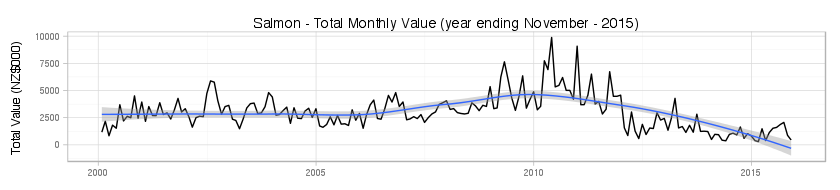
\includegraphics[scale=0.5]{../graphs/monthly_value/salmon_monthly_value.png} \
    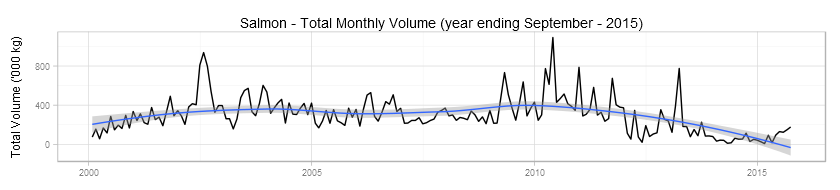
\includegraphics[scale=0.5]{../graphs/monthly_volume/salmon_monthly_volume.png} \
    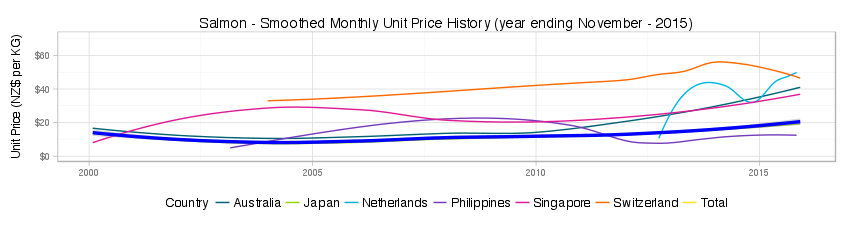
\includegraphics[scale=0.5]{../graphs/smoothed_price/salmon_smoothed_price.png} \
    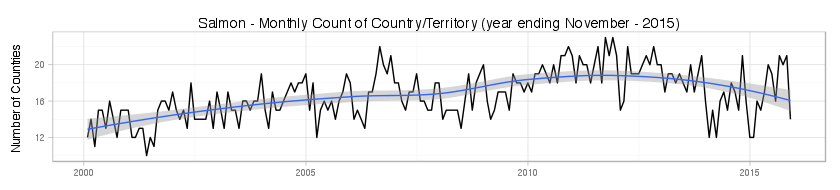
\includegraphics[scale=0.5]{../graphs/monthly_number_countries/salmon_monthly_count.png} \
    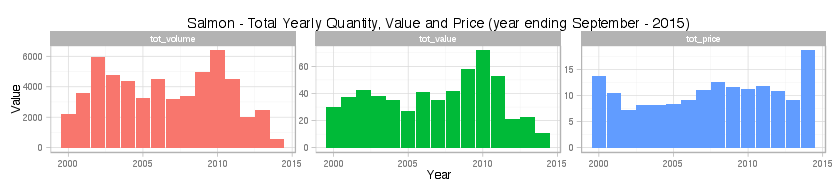
\includegraphics[scale=0.5]{../graphs/yearly_summary/salmon_yearly_summary.png} \
   \end{figure}



\footnotetext[1]{Source: Statistics New Zealand - Overseas Merchandise Trade}
\footnotetext[2]{Harmonised System Codes for Salmon starting with: 030212, 030214, 030219, 030310, 030311, 030312, 030313, 030319, 030329, 030541.}
\end{document}
